\title{Midterm 3 for Algebra-Based Physics: Electricity and Magnetism}
\author{Dr. Jordan Hanson - Whittier College Dept. of Physics and Astronomy}
\date{\today}
\documentclass[10pt]{article}
\usepackage[a4paper, total={18cm, 27cm}]{geometry}
\usepackage{outlines}
\usepackage{graphicx}
\usepackage{amsmath}
\begin{document}
\maketitle

\section{Equations and constants}

\begin{enumerate}
\item Ohm's law: $emf = IR$.
\item Definition of magnetic flux: $\phi = \vec{B} \cdot \vec{A}$.  The units are T m$^2$, which is called a Weber, or Wb.
\item Faraday's Law: $emf = -N \frac{\Delta \phi}{\Delta t}$
\item Faraday's Law using \textbf{Inductance}, M: $emf = -M \Delta I / \Delta t$.
\item Magnetic permeability: $\mu_0 = 4\pi \times 10^{-7}$ T m A$^{-1}$
\item Units of inductance: V s A$^{-1}$, which is called a Henry, or H.
\end{enumerate}

\section{Exercises}

\begin{enumerate}
\item \textbf{Chapter 23: Magnetic Induction, Faraday's Law, and AC power}
\begin{enumerate}
\item
\begin{figure}[ht]
\centering
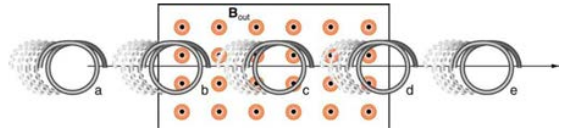
\includegraphics[width=0.6\textwidth]{movingring.png}
\caption{\label{fig:flux1} A loop of wire passes through a magnetic field.}
\end{figure}
A coil is moved through a magnetic field as shown in Fig. \ref{fig:flux1}. The field is uniform inside the rectangle and zero outside. What is the direction of the induced current (if one exists) and what is the direction of the magnetic force on the coil (if there is one) at each position shown?
\begin{itemize}
\item A: Current:$\rule{2cm}{0.15mm}$Force:$\rule{2cm}{0.15mm}$
\item B: Current:$\rule{2cm}{0.15mm}$Force:$\rule{2cm}{0.15mm}$
\item C: Current:$\rule{2cm}{0.15mm}$Force:$\rule{2cm}{0.15mm}$
\item D: Current:$\rule{2cm}{0.15mm}$Force:$\rule{2cm}{0.15mm}$
\item E: Current:$\rule{2cm}{0.15mm}$Force:$\rule{2cm}{0.15mm}$
\end{itemize}
\item Consider again the system in Fig. \ref{fig:flux1}, also known as a \textit{magnetic damper}, used to dampen the needle motion in weight scales.  The area of the loop ($N=1$ turns) is 10 cm$^2$, and the value of the B-field inside the rectangle is 0.1 T.  If it takes the loop 0.01 seconds to enter the B-field, (a) what is the induced emf? (b) If the resistance of the loop is 2$\Omega$, what is the current, according to Ohm's law? \\ \vspace{4cm}
\item 
\begin{figure}
\centering
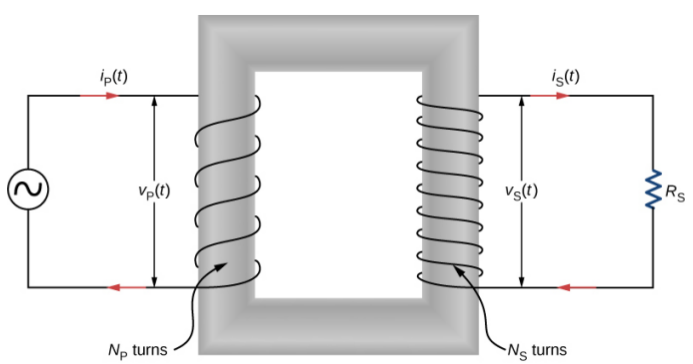
\includegraphics[width=0.45\textwidth]{transformer.png}
\caption{\label{fig:trans} (Left) A magnetic field passes through loops of wire.  (Right) The loops are stretched, reducing the area.}
\end{figure}
In Fig. \ref{fig:trans} (left) a \textit{transformer} is depicted.  The gray square represents an iron core which ensures that the magnitude of the magnetic flux through the left solenoid \textbf{is identical to} the magnetic flux on the right solenoid.  Suppose the left solenoid has $N_L = 500$ turns, and the right solenoid has $N_R = 1000$ turns.  Let the induced emf in the left solenoid be $v_L$, and the induced emf in the right solenoid be $v_R$.  Using a version of Faraday's Law, show that
\begin{equation}
\frac{v_L}{N_L} = \frac{v_R}{N_R}
\end{equation} \\ \vspace{3cm}
\item Suppose the current changes in the left solenoid of Fig. \ref{fig:trans} at a rate of 100 A s$^{-1}$, and that the inductance of the \textbf{left solenoid} is 0.1 Henries.  (a) What is the induced emf in the \textbf{left solenoid}? (b) Using the result that $\frac{v_L}{N_L} = \frac{v_R}{N_R}$, calculate the induced emf in the \textbf{right solenoid}. \\ \vspace{4cm}
\end{enumerate}
\end{enumerate}
\end{document}